\documentclass{report}
\usepackage{amsmath}
\usepackage{amsthm}
\usepackage{amsfonts}
\usepackage{mathrsfs}
\usepackage{bm}
\usepackage[usenames,dvipsnames]{xcolor}
\usepackage{tikz}
\usepackage{hyperref}

\hypersetup{
    colorlinks,
    linkcolor={red!30!black},
    citecolor={blue!50!black},
    urlcolor={blue!80!black}
}


\begin{document}



\newcommand{\vct}[1]{\mathbf{#1}}
\newcommand{\vx}{\vct{x}}
\newcommand{\vy}{\vct{y}}
\newcommand{\Z}{\mathcal{Z}}
\newcommand{\E}{\mathcal{E}}
\newcommand{\Ham}{\mathcal{H}}
\newcommand{\W}{\mathcal{W}}
\newcommand{\A}{\mathcal{A}}
\newcommand{\LL}{\mathcal{L}}
\newcommand{\var}{\mathrm{var}}
\newcommand{\com}{\mathrm{com}}

\newcommand{\llbra}{[\![}
\newcommand{\llket}{]\!]}

% annotation macros
\newcommand{\repl}[2]{{\color{gray} [#1] }{\color{blue} #2}}
\newcommand{\add}[1]{{\color{blue} #1}}
\newcommand{\del}[1]{{\color{gray} [#1]}}
\newcommand{\note}[1]{{\color{OliveGreen}\small [\textbf{Comment.} #1]}}





\title{Markov-chain Monte Carlo Simulations}
\author{ \vspace{-10ex} }
\date{ \vspace{-10ex} }


\maketitle

\abstract{
  In this note, we try to explain Markov-chain Monte Carlo simulations work.
  %
  The focus are the properties of a general transition matrix,
  and how they lead to the Perron-Frobenius theorem.
}

%\tableofcontents



\chapter{Transition matrices}



In this chapter, we shall review the basics of
Markov chains and transition matrices
and how they lead to a unique stationary distribution
(Perron-Frobenius theorem).
%
Our main source is Van Kampen\cite{vankampen},
Chapter 5.


\section{Probability distributions
and stochastic processes}



A discrete probability \emph{distribution}
is an array of $N$ numbers
\begin{equation}
  \mathbf p
  =
  (p_1, \dots, p_N),
\end{equation}
with
\begin{equation}
  p_k \ge 0,
  \qquad
  \mathrm{and}
  \qquad
  \sum_{ k = 1 }^N p_k = 1.
\label{eq:probreq}
\end{equation}

In a \emph{stochastic process},
the distribution $\mathbf p(t)$
changes with time $t$.


Now there are at least two ways of
interpreting probability.
%
\begin{enumerate}
  \item
  The frequency way:
  if I roll a dice many times,
  the frequency of me getting the number $i$
  is given by $p_i$.

  \item
  The population or ensemble way:
  if there are $10^6$ people like me,
  and everyone of them rolls a dice;
  then there are roughly $10^6 \times p_i$ of them
  getting the number $i$.

\end{enumerate}


The first way is rather clumsy
for studying stochastic processes.
%
This is because by interpreting probabilities as
frequencies, we have to image, at any given time $t$,
a \emph{repeated} experiment, which demands
another time dimension.
%
But imagining two time dimensions
can be quite stressful to the brain.
%
On the other hand,
we can think readily imagine at any time
there are $10^6$ people standing
on $N$ different sites.
Then they start to move about
among the sites as $t$ changes.
%
This makes the population interpretation
more convenient.



\section{Markov chain}




A \emph{Markov process} is special stochastic process,
in which the system has no memory.
%
Assuming discrete time, then
the distribution $\mathbf p(t+1)$ at time $t + 1$
depends only on distribution
$\mathbf p(t)$ at the previous time, $t$.
%
Usually we assume that the dependence is linear, so that
$$
  \mathbf p(t+1)
  =
  \mathbf T(t) \, \mathbf p(t).
$$
where $\mathbf T(t)$ is a $N$ by $N$ square matrix.
%
If $\mathbf T(t)$ is independent of time,
then we call this process a \emph{Markov chain}.
%
The time evolution of the probability follows
%
\begin{equation}
  \mathbf p(t+1)
  =
  \mathbf T \, \mathbf p(t),
\label{eq:mcp}
\end{equation}
%
and $\mathbf T$ is the transition matrix.


Now Eq. \eqref{eq:mcp} is a matrix equation.
In practice, we always need to write it in component form
%
\begin{equation}
  p_i(t + 1)
  =
  T_{i1} \, p_1(t)
  + \cdots +
  T_{iN} \, p_N(t)
  =
  \sum_{j = 1}^N T_{ij} \, p_j(t)
  .
\end{equation}
%
We can represent the components $T_{ij}$
graphically as follows:
%
\begin{figure}[h]
  \centering
  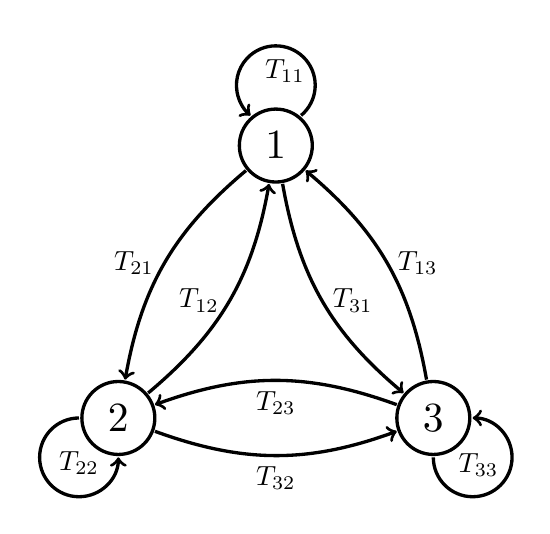
\begin{tikzpicture}
    \node[draw, circle, very thick, scale=1.5] (1) at (2, 3.46) {$1$};
    \node[draw, circle, very thick, scale=1.5] (2) at (0, 0)    {$2$};
    \node[draw, circle, very thick, scale=1.5] (3) at (4, 0)    {$3$};
    \draw[->, very thick]
        (1) edge[bend right=20] node [left]   {$T_{21}$} (2)
        (2) edge[bend right=20] node [below]  {$T_{32}$} (3)
        (3) edge[bend right=20] node [right]  {$T_{13}$} (1)
        (1) edge[bend right=20] node [right]  {$T_{31}$} (3)
        (2) edge[bend right=20] node [left]   {$T_{12}$} (1)
        (3) edge[bend right=20] node [below]  {$T_{23}$} (2)
        ;
    % self arrows
    % ++(50:5mm) shift the start point to node 1 + 5mm * (cos(50), sin(50))
    \draw [->, very thick] (1) ++(50:5mm)
        node [anchor=-70, inner sep=4mm] {$T_{11}$}
        arc (-50:230:5mm);
    % ++(180:5mm) shift the start point to node 2 + (-5mm, 0)
    \draw [->, very thick] (2) ++(180:5mm)
        node [anchor=90, inner sep=4mm] {$T_{22}$}
        arc (-270:0:5mm);
    \draw [->, very thick] (3) ++(-90:5mm)
        node [anchor=170, inner sep=3mm] {$T_{33}$}
        arc (-180:90:5mm);
  \end{tikzpicture}
\end{figure}



\section{Transition matrix}


The transition matrix

\section*{Summary}

\begin{itemize}

  \item
  A \emph{probability distribution}
  is $n$-nonnegative numbers that sum to $1$:
  $\mathbf p = (p_1, \dots, p_N)^T$,
  with $p_k \ge 0$ and $\sum_{k = 1}^N p_k = 1$.

  \item
  Each number $p_k$ can represent a frequency (time-interpretation)
  or a fraction of population (population-interpretation).

  \item
  In a \emph{stochastic process},
  the distribution changes with time.
  So the population interpretation is more useful.

  \item
  In a \emph{Markov process},
  the distribution today $\mathbf p(t)$
  determines completely the distribution tomorrow $\mathbf p(t+1)$.
  Particularly, if the dependence is linear
  and does not change with time,
  we have a \emph{Markov chain}.

  \item
  The evolution of the distribution in a Markov chain is
  $$
  p_i(t+1) = \sum_{j = 1}^N T_{ij} \, p_j(t).
  $$
  We can think $p_i$ as the population fraction
  of people living in city $i$,
  and
  $T_{ij}$ gives the fraction of people of city $j$
  traveling to city $i$ every day.
  In matrix form, we have
  $$
  \mathbf p(t+1)
  =
  \mathbf T \cdot \mathbf p(t)
  .
  $$


  \item
  The \emph{transition matrix}, $\mathbf T$,
  is made of the numbers $T_{ij}$
  $$
  \def\arraystretch{2.4}
  \mathbf T
  =
  \left(
    \begin{array}{cccc}
      T_{11}    &   T_{12}    & \dots   & T_{1N} \\
      \vdots    &   \vdots    & \ddots  & \vdots \\
      T_{N1}    &   T_{N2}    & \dots   & T_{NN}
    \end{array}
  \right).
  $$
  The first index is for the destination,
  the second for the source.

  \item
  Properties of the transition matrix.
  \begin{enumerate}
    \item
    Since each $T_{ij}$ is a fraction,
    it cannot be negative,
    $$
    T_{ij} \ge 0.
    $$

    \item
    Since the fractions of all destinations sum to $1$,
    $$
    \sum_{i = 1}^N T_{ij} = 1,
    $$
    for any $j$,
    i.e., each column of the transition matrix
    is a distribution.

    \item
    Later, we will deduce that
    there is a stationary distribution
    $\mathbf p^s = (p^s_1, \dots, p^s_N)$,
    that
    $$
    \mathbf T \cdot \mathbf p^s
    =
    \mathbf p^s.
    $$
  \end{enumerate}

  \item
  The time evolution of a Markov chain is simple
  $$
  \mathbf p(t) = \mathbf T^t \cdot \mathbf p(0)
  .
  $$
  So the distribution at day $0$
  determines all future distributions,
  and the relation is \emph{linear}.

  \item
  We can exploit the linearity by
  decomposing the initial distribution
  into a linear combination of right eigenvectors
  of $\mathbf T$.
  If
  $$
  \mathbf p(0)
  =
  c_1 \, \mathbf v_1 + \cdots + c_N \, \mathbf v_N
  ,
  $$
  then
  $$
  \mathbf p(t)
  =
  c_1 \, \lambda_1^t \, \mathbf v_1
  + \cdots +
  c_N \, \lambda_N^t \, \mathbf v_N.
  $$
  This decomposition spares us the trouble
  of matrix multiplication.

  \item
  Eigenvectors and eigenvalues.
  \begin{enumerate}
    \item
    If multiplying $\mathbf T$ on $\mathbf v$
    is equivalent to scaling $\mathbf v$,
    $$
    \mathbf T \cdot \mathbf v
    =
    \lambda \mathbf v,
    $$
    then $\mathbf v$ is a right eigenvector of $\mathbf T$,
    and $\lambda$ is the eigenvalue.

    \item
    If we are lucky, a $N$ by $N$ transition matrix
    has $N$ eigenvectors.

    \item
    If $\mathbf v$ is an eigenvector of $\mathbf T$,
    so is any nonzero multiple of $\mathbf v$.

    \item
    If $\mathbf v$ is an eigenvector of $\mathbf T$
    with eigenvalue $\lambda$,
    $\mathbf v$ is also an eigenvector of $\mathbf T^2$
    with eigenvalue $\lambda^2$, etc.

    \item
    Similarly, $\mathbf u$ is a left eigenvector of $\mathbf T$
    if $\mathbf u \cdot \mathbf T = \lambda \mathbf u$.
  \end{enumerate}

  \item
  Properties of the transition matrix.
  \begin{enumerate}
    \item
    All eigenvalues $|\lambda_k| \le 1$.

    \item
    If $\mathbf T$ is not broken, only one eigenvalue is $1.0$.
    The corresponding eigenvector is labeled as $\mathbf v_1$,
    which corresponds to the stationary distribution $\mathbf p^s$.

    \item
    $c_1 = 1$.

    \item
    All components of $\mathbf v_k$ ($k \ge 2$)
    sum to $0$.
  \end{enumerate}
\end{itemize}

\bibliographystyle{plain}
\bibliography{simul}

\end{document}
